\documentclass[12pt,twoside]{article}
\usepackage{ifxetex}
\usepackage{textpos}
\usepackage{lscape}
\usepackage{natbib}
\usepackage[a4paper,hmargin=2.8cm,vmargin=2.0cm,includeheadfoot]{geometry}
\usepackage{tabularx,longtable,multirow,subcaption,caption}
\usepackage{fancyhdr}
\usepackage{color}
\usepackage{amsmath}
\usepackage{graphicx}
\usepackage{array}
\usepackage{enumerate}
\usepackage{adjustbox}
\usepackage{url}

\usepackage{graphicx}

\makeatletter
\DeclareFontFamily{U}{tipa}{}
\DeclareFontShape{U}{tipa}{m}{n}{<->tipa10}{}
\newcommand{\arc@char}{{\usefont{U}{tipa}{m}{n}\symbol{62}}}%

\newcommand{\arc}[1]{\mathpalette\arc@arc{#1}}

\newcommand{\arc@arc}[2]{%
  \sbox0{$\m@th#1#2$}%
  \vbox{
    \hbox{\resizebox{\wd0}{\height}{\arc@char}}
    \nointerlineskip
    \box0
  }%
}
\makeatother

\newcommand{\reporttitle}{Project Title}
\newcommand{\reportauthor}{Name}

%%%%%%%%%%%%%%%%%%%%%%%%%%%%

\begin{document}
% front page
% Last modification: 2016-09-29 (Marc Deisenroth)
\begin{titlepage}

\newcommand{\HRule}{\rule{\linewidth}{0.5mm}} % Defines a new command for the horizontal lines, change thickness here


%----------------------------------------------------------------------------------------
%	LOGO SECTION
%----------------------------------------------------------------------------------------


\includegraphics[width = 4cm]{./figures/imperial}\\[0.5cm] 

\begin{center} % Center remainder of the page

%----------------------------------------------------------------------------------------
%	HEADING SECTIONS
%----------------------------------------------------------------------------------------
\textsc{\large Department of Earth Science and Engineering}\\[0.5cm] 
\textsc{\Large Imperial College London}\\[0.5cm] 

%----------------------------------------------------------------------------------------
%	TITLE SECTION
%----------------------------------------------------------------------------------------
\vspace{1.9cm}
\HRule \\[0.4cm]
{ \fontsize{20}{21} \bfseries \reporttitle}\\ % Title of your document
\HRule \\[2.5cm]
\end{center}
%----------------------------------------------------------------------------------------
%	AUTHOR SECTION
%----------------------------------------------------------------------------------------

%\begin{minipage}{0.4\hsize}
\begin{flushleft} \large
\textit{Author:}\\
\reportauthor % Your name
\end{flushleft}
\vspace{1.5cm}
\makeatletter

\noindent Supervisors: 
\vspace{0.2cm}

\noindent Github Repository: 
\vspace{0.2cm}

\noindent Email:
\vspace{0.2cm}

\noindent Date: \@date 

\vfill % Fill the rest of the page with whitespace

\begin{center}
This report is submitted as part requirement for \{Degree Title\} at Imperial College London. It is substantially the result of my own work except where indicated explicitly in the text.  The report may be freely copied and distributed provided the source is acknowledged explicitly.
\end{center}

\makeatother


\end{titlepage}


\newpage


\newpage
\tableofcontents
\thispagestyle{empty}
\newpage


% lists
\thispagestyle{empty}
\listoffigures
\listoftables
\newpage

%%%%%%%%%%%%%%%%%%%%%%%%%%%% Main document
\section*{Abstract}
\addcontentsline{toc}{section}{\protect\numberline{}Abstract}
Abstract

\section{Introduction}
Introduction


\section{Methodology}

\begin{figure*}[tbhp]
\centering
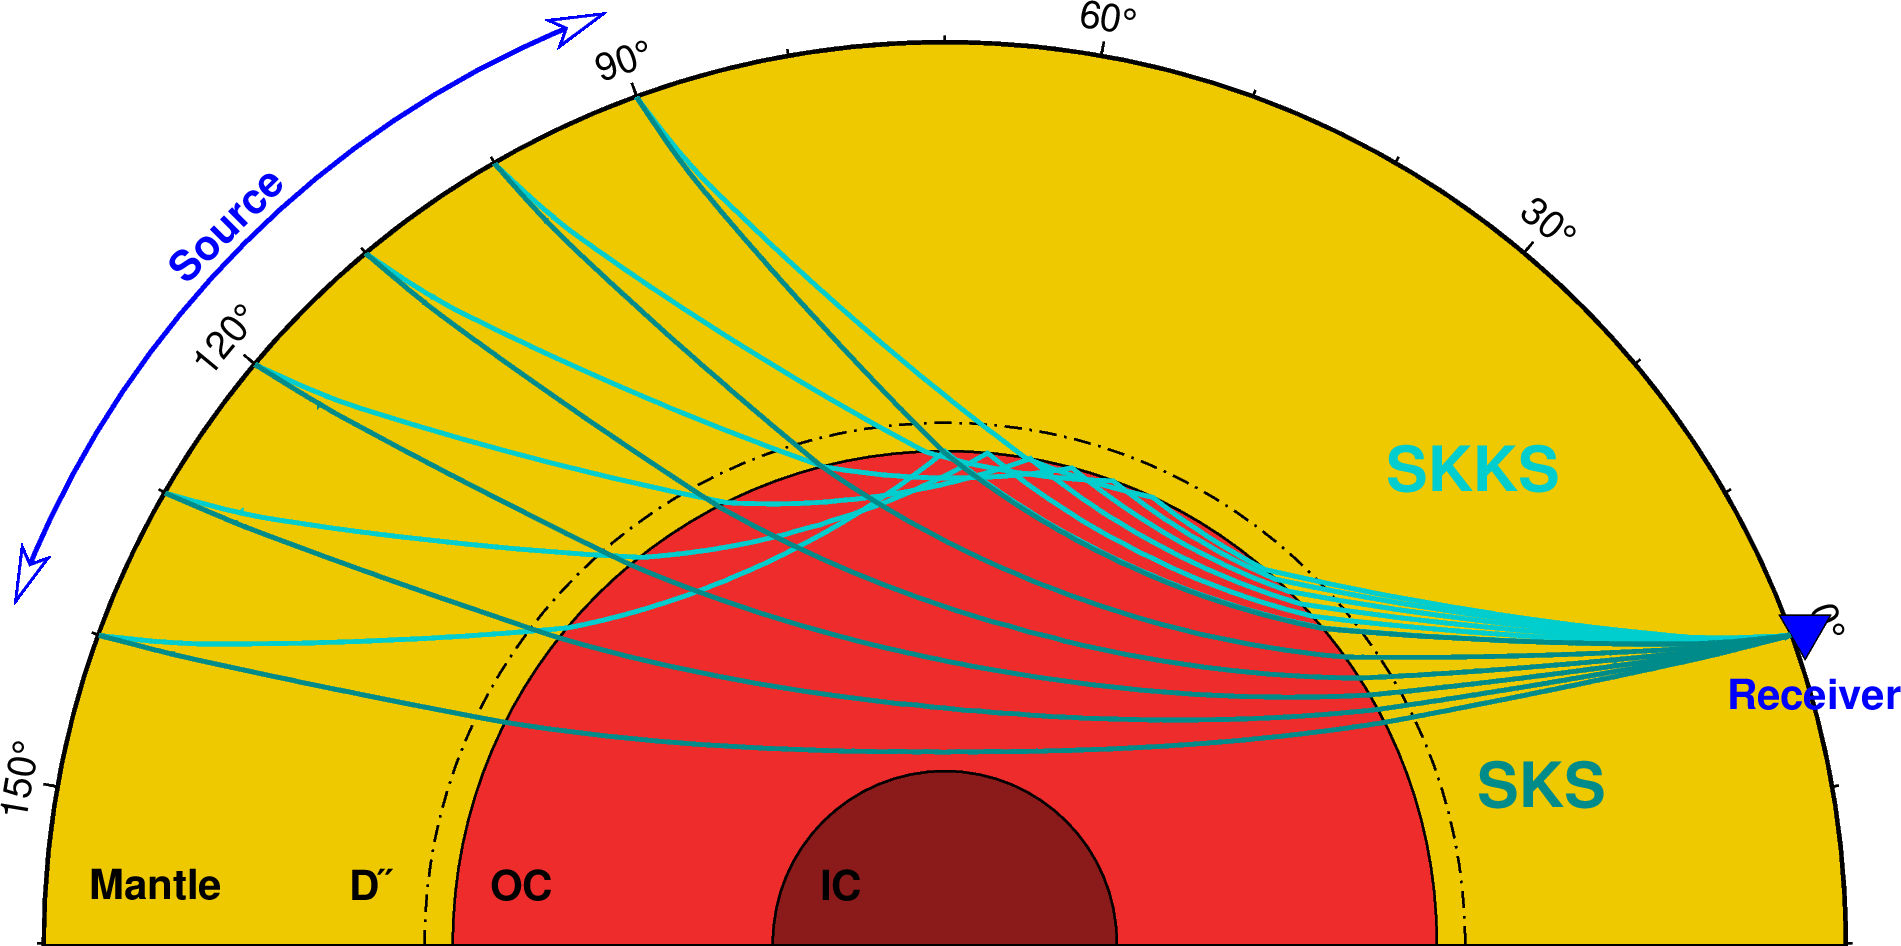
\includegraphics[width=0.65\textwidth, angle=0]{figures/raypath.png}
\caption[SKS/SKKS raypaths] {SKS and SKKS raypaths from a variety of source-receiver arc distances.}
\label{raypath}
\end{figure*}

\begin{equation}
s(H,\kappa) = \sum_{j=1}^{N} w_{1}r_{j}(t_{1}) + w_{2}r_{j}(t_{2}) - w_{3}r_{j}(t_{3}),
\label{HKobjective}
\end{equation}

where $w_{1}$, $w_{2}$, $w_{3}$ are weights, $r_{j}(t_{i})$ are the receiver function amplitudes at the predicted arrival-times of the direct $P$-to-$S$ conversion $Ps$ and subsequent reverberations $PpPs$ and $PsPs + PpSs$ respectively for the $j$th receiver function.  $N$ is the number of receiver functions used.  The predicted travel-times, $t_{i}$ are given by Equations \ref{RFStravelT1}--\ref{RFStravelT3}.

\begin{equation}
t_{1}= H\left[{\sqrt{\frac{1}{V_{S}^{2}}-p^{2}} - \sqrt{\frac{1}{V_{P}^{2}}-p^{2}}} \,\right],
\label{RFStravelT1}
\end{equation}

\begin{equation}
t_{2}=H\left[{\sqrt{\frac{1}{V_{S}^{2}}-p^{2}} + \sqrt{\frac{1}{V_{P}^{2}}-p^{2}}}\,\right],
\label{RFStravelT2}
\end{equation}

\begin{equation}
t_{3}=2H\sqrt{\frac{1}{V_{S}^{2}}-p^{2}},
\label{RFStravelT3}
\end{equation}

where $p$ is the ray parameter (skm$^{-1}$).

\subsection{Dataset}

\subsection{Model}
Model description (Fig. \ref{model_structure})

\begin{figure*}[tbhp]
\centering
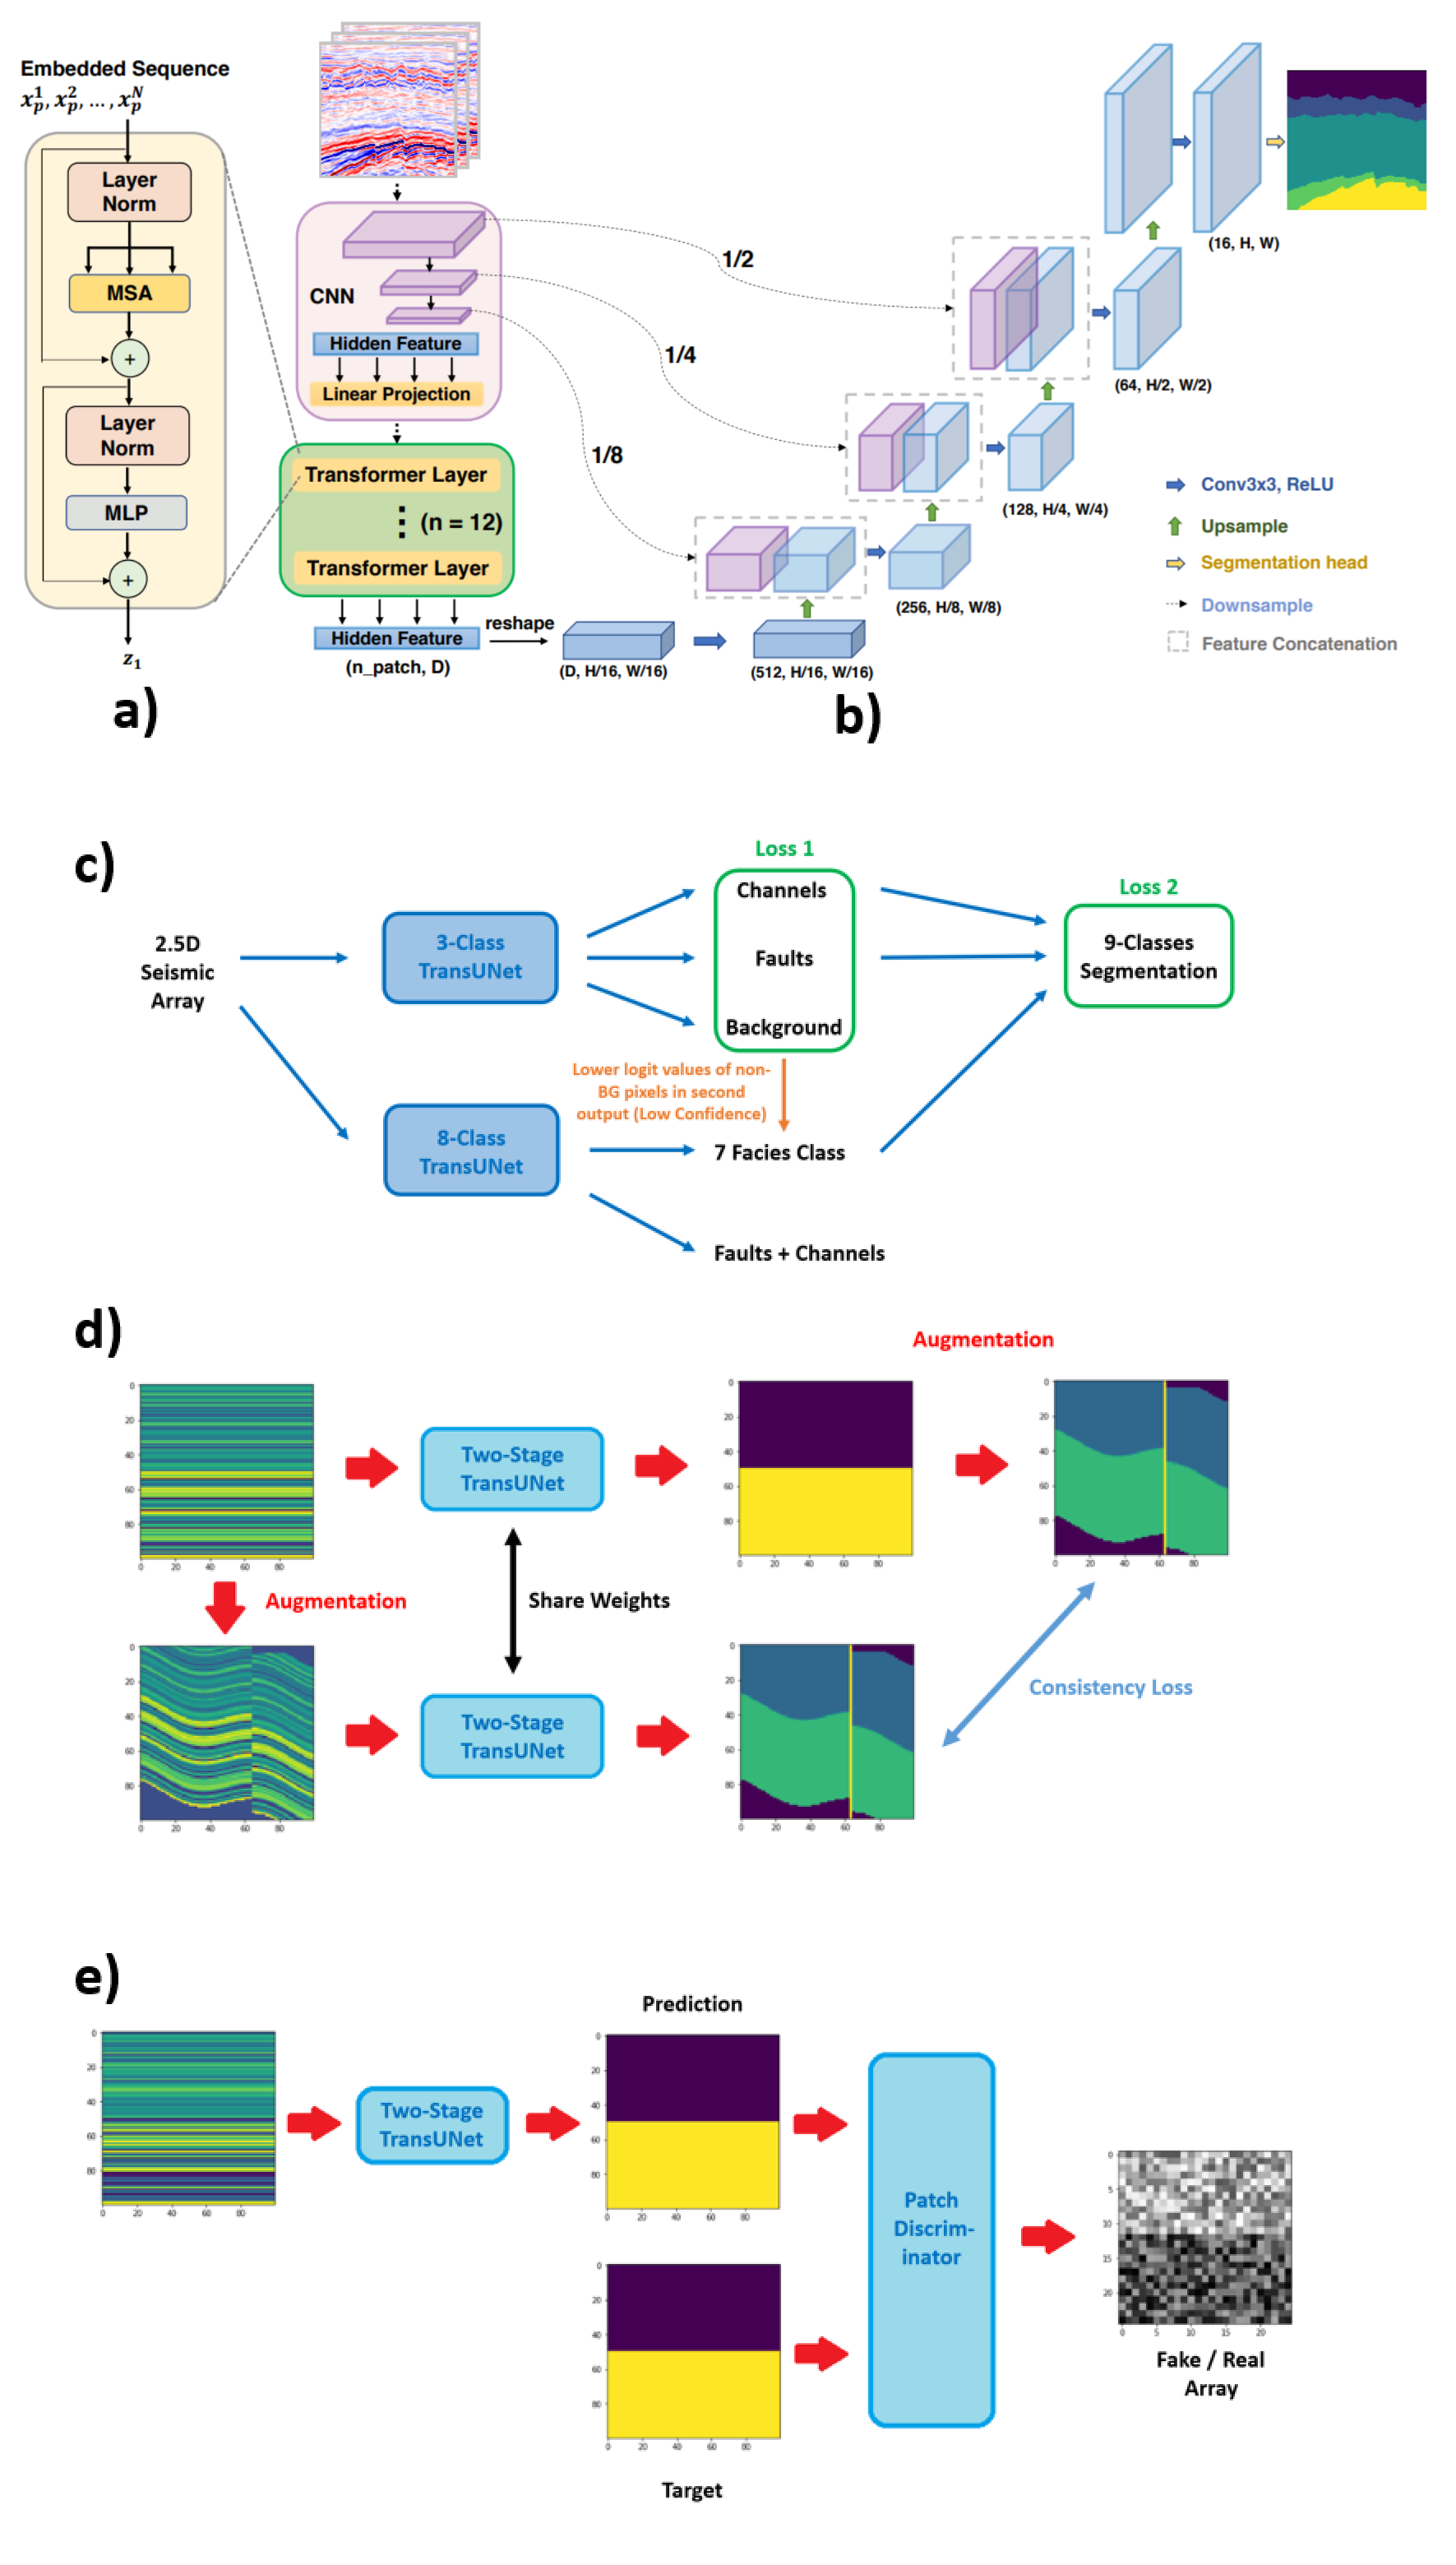
\includegraphics[width=0.4\textwidth, angle=0]{figures/dl_model_structure_full.png}
\vspace{0.5cm}
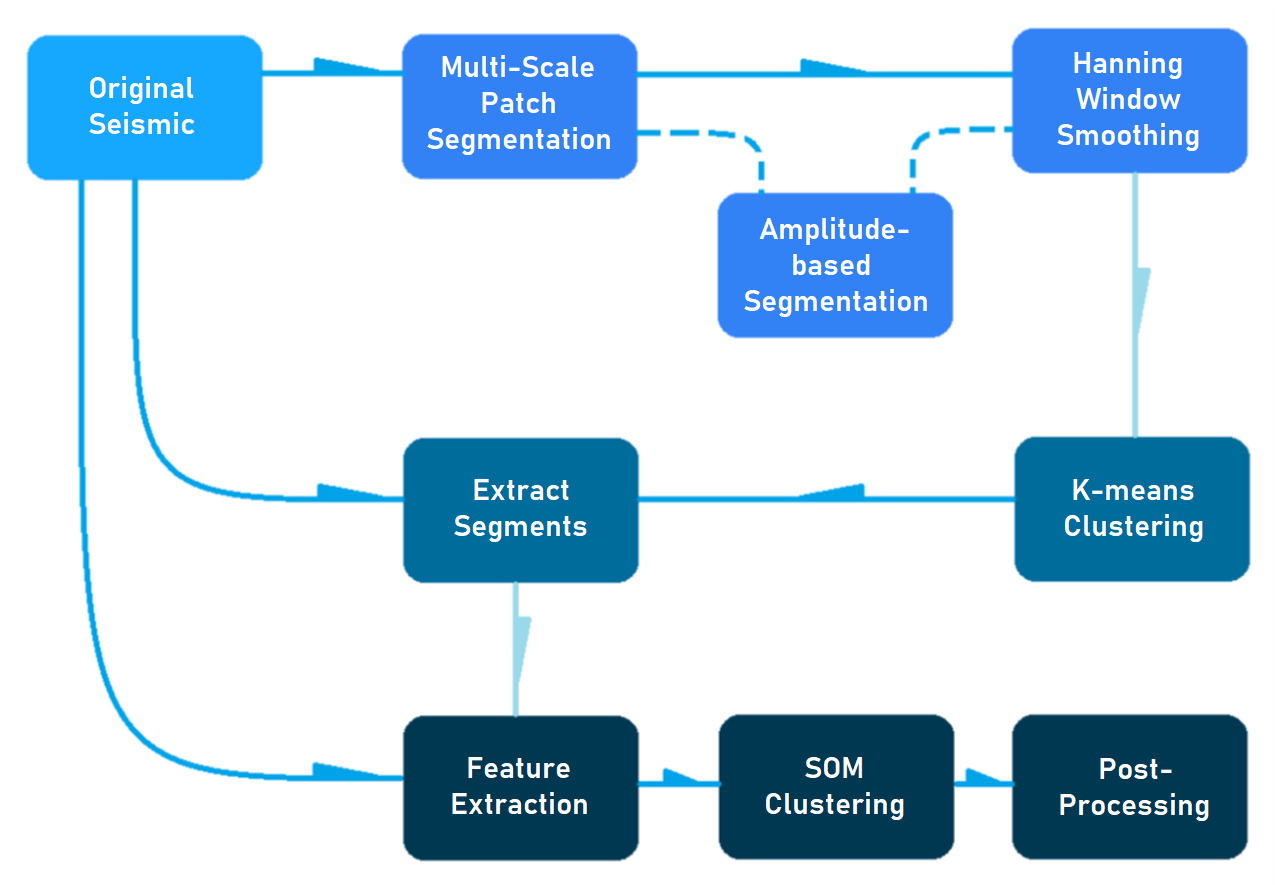
\includegraphics[width=0.75\textwidth, angle=0]{figures/unsupervised_structure.png}
\caption[Model Structure] {Top: DL structure. Bottom: ML structure. \citep{vwxg}}
\label{model_structure}
\end{figure*}

\section{Discussion}
Discussion
\newpage


\section{Conclusions}
Conclusions
\newpage

\section*{Acknowledgments}
Acknowledgements

\appendix
\section{Appendices}
\subsection{First appendix}

\begin{longtable}{|l|l|l|l|l|l|l|l|l|}
\caption[Listing of teleseismic earthquake hypocentres.]
{{\label{tabquakes}} Listing of teleseismic earthquake hypocentral information. Data come from the IRIS Data Management Center SeismiQuery website.} \\
\hline
Year & Mo. & Day & Time& Latitude & Longitude & Depth (km) & mb & Phase \\ \hline 
\endfirsthead
\caption[]{\emph{continued}}\\
\hline
Year & Mo. & Day & Time& Lat. ($^{\circ}$) & Lon. ($^{\circ}$) & Dep. (km) & mb & Phase \\ \hline 
\hline \endhead
\hline
\multicolumn{7}{l}{\emph{continued on next page}} \\
\endfoot
\hline\endlastfoot
2001 & 10 & 30 & 21:04:24.8 & 28.580$^{\circ}$N & 128.280$^{\circ}$E & 135 & 5.7 & P   \\
2001 & 11 & 14 & 09:26:10.0 & 35.950$^{\circ}$N & 090.540$^{\circ}$E &  10 & 8.0 & P,S \\
2001 & 11 & 15 & 01:03:06.1 & 01.590$^{\circ}$S  & 015.580$^{\circ}$W &  10 & 6.3 & P,S \\
2001 & 11 & 18 & 21:59:52.5 & 35.730$^{\circ}$N & 093.690$^{\circ}$E &  10 & 5.9 & P,S \\
2001 & 11 & 19 & 17:45:23.5 & 35.750$^{\circ}$N & 093.670$^{\circ}$E &  10 & 5.7 & P   \\
2001 & 11 & 20 & 21:08:18.5 & 06.880$^{\circ}$S  & 128.920$^{\circ}$E &  33 & 6.3 & P   \\
2001 & 11 & 23 & 20:43:03.6 & 36.390$^{\circ}$N & 071.510$^{\circ}$E & 106 & 6.1 & P,S \\
2001 & 11 & 25 & 14:31:57.8 & 23.030$^{\circ}$N & 125.360$^{\circ}$E &  10 & 5.6 & P   \\
2001 & 11 & 28 & 14:32:32.7 & 15.570$^{\circ}$N & 093.110$^{\circ}$W &  84 & 6.4 & P   \\
2001 & 12 & 02 & 02:47:56.3 & 12.740$^{\circ}$S  & 166.660$^{\circ}$E & 100 & 6.0 & P   \\
2001 & 12 & 02 & 13:01:53.7 & 39.400$^{\circ}$N & 141.090$^{\circ}$E & 123 & 6.5 & P,S \\
2001 & 12 & 04 & 18:09:26.7 & 18.950$^{\circ}$N & 120.240$^{\circ}$E &  33 & 5.5 & P   \\
2001 & 12 & 05 & 07:46:37.8 & 52.610$^{\circ}$S  & 018.350$^{\circ}$E &  10 & 5.7 & P   \\
2001 & 12 & 07 & 19:11:31.9 & 05.650$^{\circ}$S  & 130.740$^{\circ}$E & 111 & 5.7 & P   \\
2001 & 12 & 07 & 19:27:34.1 & 44.220$^{\circ}$S  & 168.820$^{\circ}$E &  10 & 6.1 & P   \\
2001 & 12 & 08 & 20:29:34.2 & 28.250$^{\circ}$N & 129.570$^{\circ}$E &  33 & 6.2 & P,S \\
2001 & 12 & 09 & 18:15:02.6 & 00.000$^{\circ}$N & 122.870$^{\circ}$E & 156 & 6.2 & P   \\
2001 & 12 & 12 & 12:53:18.4 & 17.190$^{\circ}$S  & 167.720$^{\circ}$E &  33 & 6.2 & P   \\
2001 & 12 & 12 & 14:02:35.1 & 42.810$^{\circ}$S  & 124.690$^{\circ}$E &  10 & 7.1 & P   \\
2001 & 12 & 13 & 13:50:46.4 & 27.040$^{\circ}$N & 044.500$^{\circ}$W &  10 & 5.7 & P   \\
2001 & 12 & 23 & 22:52:54.3 & 09.600$^{\circ}$S  & 159.530$^{\circ}$E &  16 & 7.0 & S   \\     
2001 & 12 & 27 & 10:54:51.8 & 14.650$^{\circ}$S  & 167.260$^{\circ}$E & 153 & 6.2 & P   \\
2001 & 12 & 29 & 14:32:22.6 & 06.010$^{\circ}$S  & 102.850$^{\circ}$E &  33 & 5.8 & P,S \\
2002 & 01 & 01 & 11:29:22.7 & 06.300$^{\circ}$N & 125.650$^{\circ}$E & 138 & 6.3 & P   \\
2002 & 01 & 02 & 17:22:48.8 & 17.600$^{\circ}$S  & 167.860$^{\circ}$E &  21 & 7.5 & P,S \\
2002 & 01 & 03 & 07:05:27.7 & 36.090$^{\circ}$N & 070.690$^{\circ}$E & 129 & 6.2 & P,S \\
2002 & 01 & 03 & 10:17:36.3 & 17.660$^{\circ}$S  & 168.000$^{\circ}$E &  10 & 6.7 & P,S \\
2002 & 01 & 09 & 06:45:57.5 & 38.660$^{\circ}$N & 069.900$^{\circ}$E &  33 & 5.3 & P   \\
2002 & 01 & 10 & 05:56:03.5 & 17.570$^{\circ}$S  & 167.910$^{\circ}$E &  10 & 5.7 & P   \\
2002 & 01 & 16 & 23:09:52.1 & 15.500$^{\circ}$N & 093.130$^{\circ}$W &  80 & 6.4 & P,S \\
2002 & 01 & 22 & 04:53:52.7 & 35.790$^{\circ}$N & 026.620$^{\circ}$E &  88 & 6.3 & S   \\    
2002 & 01 & 24 & 18:12:05.3 & 03.530$^{\circ}$N & 095.660$^{\circ}$E &  33 & 5.7 & P   \\
2002 & 02 & 01 & 21:55:21.0 & 45.460$^{\circ}$N & 136.720$^{\circ}$E & 355 & 6.2 & P   \\
2002 & 02 & 03 & 07:11:28.4 & 38.570$^{\circ}$N & 031.270$^{\circ}$E &   5 & 6.5 & P   \\
2002 & 02 & 03 & 09:26:43.4 & 38.630$^{\circ}$N & 030.900$^{\circ}$E &  10 & 6.0 & P   \\
2002 & 02 & 07 & 03:15:53.5 & 03.030$^{\circ}$N & 126.290$^{\circ}$E &  33 & 5.8 & P,S \\
2002 & 02 & 10 & 01:47:06.2 & 55.910$^{\circ}$S  & 029.000$^{\circ}$W & 193 & 6.0 & P   \\
2002 & 02 & 11 & 16:18:33.7 & 40.090$^{\circ}$N & 050.210$^{\circ}$E &  54 & 5.0 & P   \\
2002 & 02 & 12 & 03:27:25.9 & 23.720$^{\circ}$N & 121.560$^{\circ}$E &  54 & 5.8 & P   \\
2002 & 02 & 14 & 23:23:13.5 & 14.990$^{\circ}$N & 092.640$^{\circ}$W &  75 & 5.8 & P   \\
2002 & 02 & 24 & 02:24:31.6 & 05.650$^{\circ}$S  & 130.750$^{\circ}$E & 109 & 5.6 & P   \\
2002 & 03 & 03 & 12:08:07.8 & 36.430$^{\circ}$N & 070.440$^{\circ}$E & 209 & 6.3 & P   \\
2002 & 03 & 03 & 12:08:19.7 & 36.500$^{\circ}$N & 070.480$^{\circ}$E & 225 & 7.4 & P   \\
2002 & 03 & 05 & 21:16:09.1 & 06.030$^{\circ}$N & 124.250$^{\circ}$E &  31 & 7.5 & P   \\
2002 & 03 & 07 & 07:10:13.5 & 01.320$^{\circ}$S  & 024.480$^{\circ}$W &  10 & 5.1 & P,S \\
2002 & 03 & 08 & 18:27:53.2 & 05.870$^{\circ}$N & 124.270$^{\circ}$E &  23 & 6.0 & P   \\
2002 & 03 & 09 & 12:27:11.2 & 56.020$^{\circ}$S  & 027.330$^{\circ}$W & 118 & 6.0 & P   \\
2002 & 03 & 11 & 01:46:20.7 & 30.600$^{\circ}$N & 141.570$^{\circ}$E &  33 & 5.9 & P,S \\
2002 & 03 & 17 & 03:37:19.9 & 00.680$^{\circ}$N & 122.320$^{\circ}$E &  79 & 5.8 & P   \\
2002 & 03 & 17 & 19:33:33.8 & 45.220$^{\circ}$S  & 035.110$^{\circ}$E &  10 & 6.0 & P,S \\
2002 & 03 & 19 & 22:14:15.0 & 06.490$^{\circ}$S  & 129.900$^{\circ}$E & 148 & 6.1 & P,S \\
2002 & 03 & 22 & 17:36:59.2 & 04.590$^{\circ}$N & 126.320$^{\circ}$E &  76 & 5.7 & P   \\
2002 & 03 & 23 & 05:15:51.4 & 01.390$^{\circ}$N & 128.110$^{\circ}$E & 115 & 5.7 & P   \\
2002 & 03 & 25 & 14:56:33.8 & 36.060$^{\circ}$N & 069.320$^{\circ}$E &   8 & 6.2 & P,S \\
2002 & 03 & 26 & 03:45:48.7 & 23.350$^{\circ}$N & 124.090$^{\circ}$E &  33 & 6.6 & P,S \\
2002 & 03 & 27 & 08:52:52.3 & 36.020$^{\circ}$N & 069.340$^{\circ}$E &  10 & 5.9 & P   \\
2002 & 03 & 28 & 04:56:22.4 & 21.660$^{\circ}$S  & 068.330$^{\circ}$W & 125 & 6.5 & S   \\ 
2002 & 03 & 31 & 06:52:50.5 & 24.280$^{\circ}$N & 122.180$^{\circ}$E &  32 & 7.4 & P,S \\
2002 & 03 & 31 & 22:49:09.6 & 53.880$^{\circ}$N & 035.370$^{\circ}$W &  10 & 5.2 & P   \\
2002 & 04 & 10 & 00:13:43.2 & 44.130$^{\circ}$S  & 015.990$^{\circ}$W &  10 & 5.4 & P   \\
2002 & 04 & 10 & 10:04:50.7 & 44.180$^{\circ}$S  & 015.860$^{\circ}$W &  10 & 5.3 & P   \\
2002 & 04 & 10 & 21:47:22.0 & 43.990$^{\circ}$S  & 015.910$^{\circ}$W &  10 & 5.2 & P   \\
2002 & 04 & 12 & 04:00:23.7 & 35.960$^{\circ}$N & 069.420$^{\circ}$E &  10 & 5.9 & P,S \\
2002 & 04 & 12 & 16:26:01.6 & 35.880$^{\circ}$N & 069.260$^{\circ}$E &  10 & 4.9 & P   \\
2002 & 04 & 14 & 04:05:24.0 & 07.320$^{\circ}$N & 126.660$^{\circ}$E &  33 & 5.6 & P   \\
2002 & 04 & 18 & 14:17:23.9 & 60.660$^{\circ}$S  & 025.840$^{\circ}$W &  10 & 5.8 & P   \\
2002 & 04 & 26 & 16:06:07.0 & 13.090$^{\circ}$N & 144.620$^{\circ}$E &  85 & 7.1 & S   \\
2002 & 05 & 12 & 23:12:52.9 & 01.140$^{\circ}$S  & 127.090$^{\circ}$E &  33 & 5.9 & S   \\
2002 & 05 & 13 & 19:54:43.1 & 19.140$^{\circ}$N & 121.240$^{\circ}$E &  33 & 5.5 & P   \\
2002 & 05 & 13 & 19:57:22.9 & 19.120$^{\circ}$N & 121.240$^{\circ}$E &  33 & 5.8 & P   \\
2002 & 05 & 14 & 14:19:03.4 & 03.510$^{\circ}$N & 125.380$^{\circ}$E &  33 & 5.5 & P   \\
2002 & 05 & 14 & 14:56:49.4 & 36.500$^{\circ}$S  & 078.740$^{\circ}$E &  10 & 4.9 & P   \\
2002 & 05 & 14 & 16:56:10.4 & 36.520$^{\circ}$S  & 078.930$^{\circ}$E &  10 & 6.3 & P,S \\
\end{longtable}
\newpage

\newpage
\subsection{Second appendix}
More stuff here...

%%%%%%%%%%%%%%%%%%% %%%%%%%%%%%%%%%%%%% %%%%%%%%%%%%%%%%%%% %%%%%%%%%%%%%%%%%%% 
%%%%%%%%%%%%%%%%%%% Now adding the bibliography at the end. %%%%%%%%%%%%%%%%%%% 
%%%%%%%%%%%%%%%%%%% %%%%%%%%%%%%%%%%%%% %%%%%%%%%%%%%%%%%%% %%%%%%%%%%%%%%%%%%% 

\newpage

\bibliographystyle{agufull08}
\addcontentsline{toc}{section}{\protect\numberline{}References}
\bibliography{zotero_clean}

\end{document}



